\subsection{Kort}
	Dette afsnit vil indeholde en gennem gang af design, grafisk bruger interface og implentering af Kort activityen til android applikationen
	
	\subsubsection{Design}

	\subsubsection{Grafisk Bruger Interface}
	Her vises guien for kort delen af applikationen.
	\begin{figure} [!ht]
		\begin{center}
			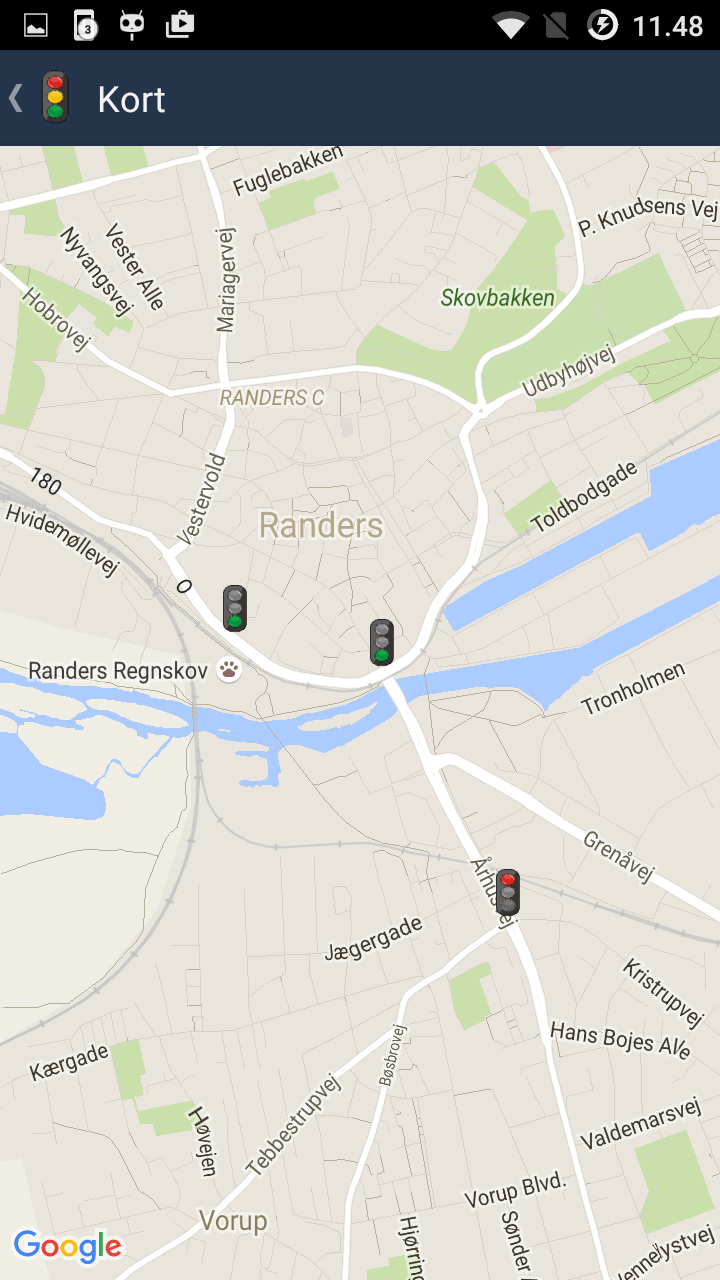
\includegraphics[height=10cm]{Android/Billeder/AndroidMap}
		\end{center}
		\caption{Map på android appliakationen}
		\label{fig:Map på android appliakationen}
	\end{figure} \\
	Man har mulighed for at vælge kort i menuen på Home page. Vælger man denne funktion kommer man ind på en skærm som ser ud som den ovenstående.\\
	Her får man et kort frem af Randers by, hvor at der er påsat markers for lyskrydsene i Randers kommune. Man kan ud fra farven på traffiklys ikonet se hvilken status lyskrydset her. Er ikonet grønt er alt som det skal være, hvorimod hvis den er rød er der en fejl i installationen.
		
	\subsubsection{Implementering}
	
	\pagebreak